\vspace*{-0.4cm}
\section{Introduction}
\label{sec:introduction}

\begin{figure}
    \centering
    \vskip -0.25cm
    \begin{subfigure}[t]{0.5\textwidth}
        \centering
        \hspace*{-0.5cm}
        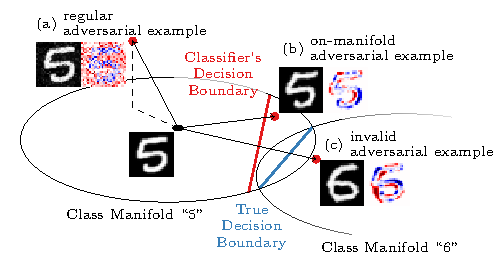
\includegraphics[width=0.9\textwidth]{introduction_b.pdf}
    \end{subfigure}
    \vskip -8px
    {\color{black!75}\noindent\rule{0.45\textwidth}{0.4pt}}
    \vskip 4px
    \begin{subfigure}[t]{0.5\textwidth}
        \centering
        \hskip -0.5cm
        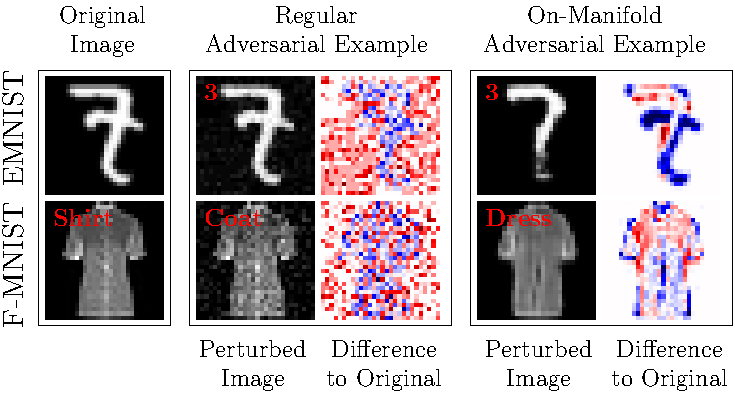
\includegraphics[width=0.8\textwidth]{introduction_a.pdf}
    \end{subfigure}
    \vskip -6px
    \caption{Adversarial examples, and their (normalized) difference to the original image, in the context of the underlying manifold, \eg, class manifolds ``5'' and ``6'' on \MNIST \cite{CohenARXIV2017}, allow to study their relation to generalization. Regular adversarial examples are not constrained to the manifold, \cf (a), and often result in (seemingly) random noise patterns; in fact, we show that they leave the manifold. However, adversarial examples on the manifold can be found as well, \cf (b), resulting in meaningful manipulations of the image content; however, care needs to be taken that the actual, true label \wrt the manifold does not change, \cf (c).}
    \label{fig:introduction}
    \vskip -2px
\end{figure}

Adversarial robustness describes a deep network's ability to defend against adversarial examples \cite{SzegedyARXIV2013}, imperceptibly perturbed images causing mis-classification. These adversarial attacks pose severe security threats, as demonstrated against Clarifai.com~\cite{LiuICLR2017,BhagojiARXIV2017b} or Google Cloud Vision~\cite{IlyasICML2018}. Despite these serious risks, defenses against such attacks have been largely ineffective; only adversarial training, \ie, training on adversarial examples \cite{MadryICLR2018,GoodfellowARXIV2014}, has been shown to work well in practice \cite{AthalyeARXIV2018,AthalyeARXIV2018b} -- at the cost of computational overhead and reduced accuracy. Overall, the problem of adversarial robustness is left open and poorly understood -- even for simple datasets such as \MNIST \cite{CohenARXIV2017} and \FashionMNIST \cite{XiaoARXIV2017}.

The phenomenon of adversarial examples itself, \ie, their mere existence, has also received considerable attention. Recently, early explanations, \eg, attributing adversarial examples to ``rare pockets'' of the classification surface \cite{SzegedyARXIV2013} or linearities in deep networks \cite{GoodfellowARXIV2014}, have been superseded by the manifold assumption \cite{GilmerICLRWORK2018,TanayARXIV2016}: adversarial examples are assumed to leave the underlying, low-dimensional but usually unknown data manifold. \red{However, only \cite{SongICLR2018} provide experimental evidence supporting this assumption.} Yet, on a simplistic toy dataset, Gilmer \etal \cite{GilmerICLRWORK2018} also found adversarial examples on the manifold, as also tried on real datasets \cite{SongARXIV2018,BrownARXIV2018,ZhaoICLR2018}, rendering the manifold assumption questionable. Still, the manifold assumption fostered research on novel defenses \cite{IlyasARXIV2017,SamangoueiICLR2018,SchottARXIV2018}.

Beyond the existence of adversarial examples, their relation to generalization is an important open problem. Recently, it has been argued \cite{TsiprasARXIV2018,SuARXV2018} that there exists an inherent trade-off, \ie, robust and accurate models seem impossible. While Tsipras \etal \cite{TsiprasARXIV2018} provide a theoretical argument on a toy dataset, Su \etal \cite{SuARXV2018} evaluate the robustness of different models on ImageNet \cite{RussakovskyIJCV2015}. However, these findings have to be questioned  given the results in \cite{GilmerICLRWORK2018,RozsaICMLA2016} showing the opposite, \ie, better generalization helps robustness.

In order to address this controversy, and in contrast to \cite{TsiprasARXIV2018,SuARXV2017,RozsaICMLA2016}, we consider adversarial robustness in the context of the underlying manifold. In particular, to break the hypothesis down, we explicitly ask whether adversarial examples leave, or stay on, the manifold. On \MNIST, for example, considering the class manifolds for ``5'' and ``6'', as illustrated in \figref{fig:introduction}, adversarial examples are not guaranteed to lie on the manifold, \cf \figref{fig:introduction} (a). Adversarial examples can, however, also be constrained to the manifold, \cf \figref{fig:introduction} (b); in this case, it is important to ensure that the adversarial examples do not actually change their label, \ie, are more likely to be a ``6'' than a ``5'', as in \figref{fig:introduction} (c). For clarity, we refer to unconstrained adversarial examples, as illustrated in \figref{fig:introduction} (a), as \emph{regular adversarial examples}; in contrast to adversarial examples constrained to the manifold, so-called \emph{on-manifold adversarial examples}.

\myparagraph{Contributions:} Based on this distinction between regular robustness, \ie, against regular, unconstrained adversarial examples, and on-manifold robustness, \ie, against adversarial examples constrained to the manifold, we show:
\begin{enumerate}[itemsep=0ex,topsep=2px,parsep=2px]
    \item regular adversarial examples leave the manifold;
    \item adversarial examples constrained to the manifold, \ie, on-manifold adversarial examples, exist and can be computed using an approximation of the manifold;
    \item on-manifold robustness is essentially generalization;
    \item \red{and regular robustness and generalization are not necessarily contradicting goals, \ie, for any arbitrary but fixed model, better generalization through additional training data does not worsen robustness.}
\end{enumerate}
\noindent \red{We conclude that both robust and accurate models are possible and can, \eg, be obtained through adversarial training on larger training sets.} Additionally, we propose on-manifold adversarial training to boost generalization in settings where the manifold is known, can be approximated, or invariances of the data are known. We present experimental results on a novel MNIST-like, synthetic dataset with known manifold, as well as on \MNIST \cite{CohenARXIV2017}, \FashionMNIST \cite{XiaoARXIV2017} and \Celeb \cite{LiuICCV2015}. \red{We will make our code and data publicly available.}